%*****************************************
% Justin Ragatz
%
% 19 April 2016
%
% OnRamp Module for Monte Carlo Methods
%*****************************************

% Document options
\documentclass[a4paper, 11pt]{article}

\makeatletter
% Change the square brackets for each bibliography item from '[1]' to '1.'
\renewcommand\@biblabel[1]{\textbf{#1.}}

% Reduce the space between items in the itemize and enumerate environments and the bibliography
\renewcommand{\@listI}{\itemsep=0pt}

% Decimal section numbers
\renewcommand*\thesection{\arabic{section}.0}
\renewcommand*\thesubsection{\arabic{section}.\arabic{subsection}}

% Custom title
\renewcommand{\maketitle}
{
	\begin{flushright}
	{\LARGE\@title}

	\vspace{20pt}

	{\large\@author}

	\end{flushright}
}
\makeatother

% Header options
\usepackage{fancyhdr}
\pagestyle{fancy}
\fancyhf{}
\rhead{\small Monte Carlo Methods}
\lhead{\small OnRamp Module}
\rfoot{\small Page \thepage}

% Image options
\usepackage{graphicx}
\usepackage{float}
\usepackage{wrapfig}
\graphicspath{{images/}}

% Font options
\usepackage{mathpazo}
\usepackage[scaled]{helvet}
\usepackage{courier}
\normalfont
\usepackage[T1]{fontenc}
\usepackage{microtype}
\usepackage{url}
\urlstyle{same}
\usepackage{algpseudocode}
\usepackage{algorithm}
\usepackage{listings}
\usepackage{color}

% Title
\title{\textbf{Monte Carlo Methods}}
\author{\textsc{Justin Ragatz}}

\lstdefinestyle{customc}{
	belowcaptionskip=1\baselineskip,
	breaklines=true,
	frame=lines,
	xleftmargin=\parindent,
	language=C,
	showstringspaces=false,
	basicstyle=\footnotesize\ttfamily
}

\lstdefinestyle{customasm}{
	belowcaptionskip=1\baselineskip,
	frame=L,
	xleftmargin=\parindent,
	language=[x86masm]Assembler,
	basicstyle=\footnotesize\ttfamily
}

\lstset{escapechar=@,style=customc}

\begin{document}

% Title
\maketitle
\bigskip

% Module summary
\begin{description}
  \item[Summary] Use Monte Carlo methods to approximate the probabilities of various outcomes in card games and the roulette wheel.
  \item[Duration] 5 hours
  \item[Prerequisites] Familiarity with for-loops, rand(), and 1D arrays.
\end{description}

% Overview
\section{Overview}

Monte Carlo methods are a class of computational algorithms that use repeated random sampling to obtain numerical results. Typically, a single workhorse for-loop is used to generate the repeated and independent simulations. Because the numerous simulations are independent of each other, they can be easily split among multiple processing units. A problem such as this, where little effort is required to separate the problem into parallel tasks is known as "embarrassingly parallel". Thus, Monte Carlo methods are a convenient vehicle to introduce parallel concepts at the CS1/CS2 level. 

By exposing students to parallel solutions at the introductory level, they come to expect parallel solutions throughout the curriculum. In particular, students are not overwhelmed by the sudden introduction of concurrency and similar topics in senior-level coursework. Upon completion of this module, students should be able to: 1) Identify embarrassingly parallel problems 2.) Understand the real-life applications of stochastic methods 3.) Explain at a high level how OpenMP works, and 4.) Measure the scalability of a parallel application.

Much of the material in this module has been adapted from the Monte Carlo Methods module written by Devin Bjelland and Libby Shoop\cite{website:shoop:2015}.

% Introducation to the problem
\section{Introduction to Monte Carlo Methods}

Monte Carlo methods are often employed when there is not a closed form or deterministic solution to the underlying problem. As this sort of problem is quite common, Monte Carlo methods are used in a wide variety of fields from computational chemistry to finance. While these topics are important, the typical CS1/CS2 student may be more interested in the more intriguing application of Monte Carlo methods to gambling and card games. The well known games of roulette and poker will both be used as the basis for the exercises in this module.

\subsection{How Computers Generate Random Numbers}

Algorithms that implement Monte Carlo methods require a source of randomness. When writing a serial algorithm, we can simply use the standard random number generator, for example, rand() in C. Computers (unless specifically fitted with a chip which gathers randomness from some other source) cannot produce true random numbers. Rather, the standard library random number generator takes some relatively random 32-bit or 64-bit integer input, called the seed, and transforms it sequentially to produce a stream of pseudo-random numbers. A random number generator is created with the seed as input to a function called srand(), and each time a new random number is requested using the rand() function, the integer pattern is changed to produce a new number. The sequence of numbers produced by such a pseudo-random number generation algorithm try to approximate a uniform distribution of numbers, each one statistically independent from the others.

However, it is important to realize that for a given input seed a pseudo-random number generator function such as rand() creates the same sequence of numbers every time. In C and C++, the function time() is often used to create the seed integer, because it returns the number of seconds since January 1, 1970. When running a sequential program multiple times, this seed would be different each time the program was run and the pattern of random numbers generated would be different.

\subsection{Testing out random number generators}

A simple way to test a random number generator is to simulate flipping a coin for a large number of trials.

We will use srand() to seed our random number generator with a large integer and then make numerous calls to rand\_r() to obtain a series of random integers. If the integer is even, we call it a "head", otherwise it is a "tail". This code sets up trials of coin flips with ever increasing numbers of flips. It also calculates the Chi Square statistic using the number of heads and tails. Generally, a Chi-Square value of 3.8 or less is considered a good random distribution of "heads" and "tails". We want to verify that the random number generator provides such an independent distribution. 

\paragraph{Coding Exercise:}
Please refer to the sequential coin-flipping program in the accompanying files to run this test for yourself.

% Introduction to Parallelism
\section{Introduction to Parallelism}

We can make our coin flipping simulation run much faster by making use of the multiple cores available in modern CPUs. This type of code is known as parallel code, because we can designate portions of our program to run concurrently in parallel on different cores, computing part of the overall solution. In the case of flipping a coin, we can intuitively sense that it might be simple enough to designate that each core we have available could carry out some portion of the flips independently while other cores were taking care of the rest of the needed flips.

\subsection{Parallel Code with Threads}

A common mechanism for running code on multiple cores simultaneously is to start threads that can execute part of our code independently and in parallel on separate cores, sharing data values in memory if needed. When a program using threads begins execution, it is always running on a single main thread, which we conceptually label as thread 0. Then within the code we can designate that more threads should start executing in parallel along with thread 0. We call a point in the code where multiple threads are executing concurrently a fork of those threads. Then when they are done executing, we think of them as joining back with the main thread. Conceptually, this looks like this:

\begin{figure}[h]
	\begin{center}
		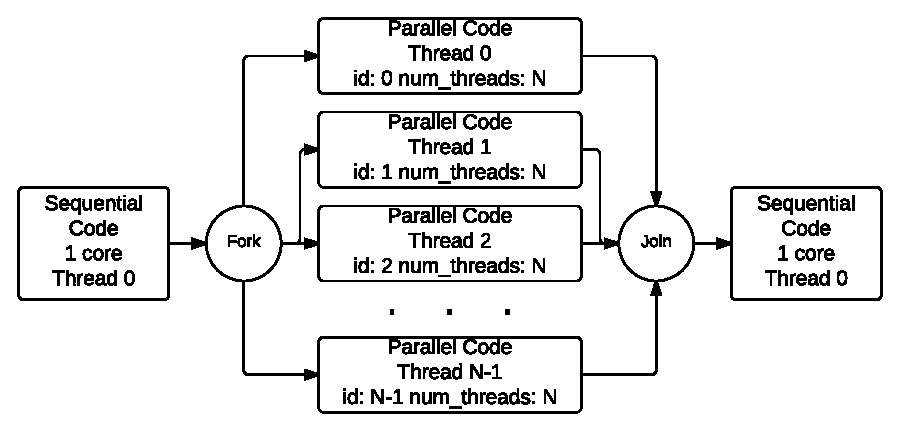
\includegraphics[width=0.9\textwidth]{figure1.pdf} 
		\caption{Fork and Join}
	\end{center}
\end{figure}

\subsection{Introduction to OpenMP}

While there are many thread libraries available, pthreads is the basic library for threading in C. A more convenient way to get started using threads is to use OpenMP, which is built into several popular C compilers as a means to compile high-level directives into threaded code using an underlying threads library. Let's take a look at a very simple example of how this works:

\pagebreak
%
% Illustration of OpenMP thread forking
%
\begin{lstlisting}[language=C]
01. #include<stdio.h>
02. #include<omp.h>
03. 
04. int main (int argc, char* argv[]) {
05.     #pragma omp parallel
06.     {
07.         int id = omp_get_thread_num();
08.         int n_threads = omp_get_num_threads();
09.         printf("Hello from thread %d of %d\n", 
10.                id, n_threads);
11.     }
12.     return 0;
13. }
\end{lstlisting}

Line 5 of this code illustrates how we can designate that the main thread 0 should fork and start multiple threads simultaneously. The code within the block following that line and between the curly braces will execute independently on each thread. Lines 7 and 8 illustrate functions that are available as part of the OpenMP library, which was included on line 2. There are several other functions available, most notably one that lets you set the number of threads to use, omp\_set\_num\_threads(), and one that lets you time your threaded code, omp\_get\_wtime(), to see how much faster it performs.

\pagebreak

\subsection{For-loop parallelization}

In a great deal of code examples, much of the work being performed can be found within for loops that are performing a large number of iterations, such as the coin-flipping example in the previous section. A well-used pattern in parallel programming is to split the work being done in these loops across multiple forked threads. OpenMP has a pragma for designating this in the code. Here is a simple example:

\begin{lstlisting}[language=C]
01. #include<stdio.h>
02. #include<omp.h>
03. 
04. int main (int argc, char* argv[]) {
05.     int n_threads = 16;
06.     int i;
07.
08.     #pragma omp parallel for num_threads(n_threads)
09.     for (i = 0; i < n_threads; i++) { 
10.         int id = omp_get_thread_num();
11.         printf("Thread %d performed iteration %d \n", id, i);
12.     }
13.     return 0;
14. }
\end{lstlisting}

In this example, we set up a very small number of repetitions of the loop, simply to illustrate how forking threads and running the loop iterations works. The OpenMP pragma on line 8 is asking the compiler to set up an equal distribution of work for each thread, which will take place like this for the 4 threads and 16 repetitions of the for loop.

\pagebreak
\subsection{Coin-flipping Revisted}

Now that we know a bit about how OpenMP works to provide threads that run code in parallel, let's look at how we can update our coin-flipping example.

\begin{lstlisting}[language=C]
01. #pragma omp parallel for
02.     num_threads(n_threads)
03.     default(none)
04.     private(n_flips, seed)
05.     shared(trial_flips)
06.     reduction(+:n_heads, n_tails)
07.     for (n_flips = 0; n_flips < trial_flips; n_flips++) {
08.         #pragma omp parallel for num_threads(n_threads)
09.             for (i = 0; i < n_threads; i++) { 
10.                 // Flip coin and increment the appropriate
11.                 // counter, heads or tails.
12.             }
\end{lstlisting}

Similar to the last example we are using the $parallel for$ directive; however, we have also introduced many other useful directives including:

\begin{itemize}
\item $default()$ designates that all variables in the loop will be defined as either private within each thread or shared between the threads by the next three directives.

\item $private()$ designates that each thread will keep its own private copy of a variable and update it independently.

\item $shared()$ designates that a variable is shared by all of the threads.

\item $reduction()$ OpenMP will have each thread keep a private copy of these variables while they execute their portion of the loop. Then, when they join back after they have finished, each thread's private sum is added to an overall sum and stored in thread 0's copy of the variable.
\end{itemize}

\paragraph{Coding Exercise:}
Please refer to the parallel coin-flipping program in the accompanying files to run this program for yourself.

\pagebreak
% Experimenting with the code
\section{Experimenting with the code}

\subsection{Roulette Simulation}

An American Roulette wheel has 38 slots: 18 are red, 18 are black, and 2 are green, which the house always wins. When a person bets on either red or black, the odds of winning are 18/38, or 47.37\% of the time.

Our next is example is a simulation of spinning the Roulette wheel. We have a main simulation loop that is similar to the coin-flipping example. The code for determining a win on each spin is more involved than flipping a coin, and the sequential version, roulette\_simulation\_seq.c is decomposed into several functions. Look at this original code file to see how we run the simulations using increasing numbers of random spins of the wheel.

The function that actually runs a single simulation of the roulette wheel, called spin\_red(), is quite simple. It generates a random number to represent the slot that the ball ends up in and gives a payout according to the rules of Roulette.

\lstset{language=C}
\begin{lstlisting}[frame=single]
int spin_red(int bet, unsigned int *seed) {
    int payout;
    int slot = rand_int_between(1, 38, seed);

    if (slot <= 18)      /*spin was red   - win      */
        payout = bet;
    else if (slot <= 36) /*spin was black - lose all */
        payout = -bet;
    else                 /*spin was green - lose half*/
        payout = -(bet/2);
        
    return payout;
}
\end{lstlisting}

\pagebreak

\subsection{Roulette Simulation with Parallelism}

We add OpenMP parallelism as in the coin flip example, by running the loop of random spins for each trial on several threads. This code is located in the roulette\_simu\_omp.c file.

\lstset{language=C}
\begin{lstlisting}[frame=single]
int getNumWins(int numSpins, unsigned int seed) {
    int wins = 0;   /* our counter      */
    int spin;       /* loop control var */
    int myBet = 10; /* bet per spin     */

    #pragma omp parallel for num_threads(nThreads)
        default(none)
        shared(numSpins, myBet)
        private(spin, seed)
        reduction(+:wins)
        for (spin=0; spin < numSpins; spin++)
            if (spinRed(myBet, &seed) > 0) /* winner */
                wins++;  
    return wins;
}
\end{lstlisting}

Both num\_spins and my\_bet are shared between threads while spin is the loop index and unique to each thread. When using rand\_r() as the thread-safe random number generator in linux, the seed should be private to each thread also. Like the previous example, we combine the partial results from each thread with reduction(+:wins).

\subsection{Drawing Four Cards of the Same Suit}

Now let's turn our attention to the card game of Poker. In the next example, we will examine the probability that given a random hand of 5 cards, four cards will each have a different suit.

We represent the deck of cards as an array of integers. The function for simulating deck shuffling is not the most efficient, but it mimics how a traditional "fan" shuffle actually works. We also have helper functions for initializing a deck, drawing a hand, and checking if the hand has four cards of the same suit. The accompanying code is located in the draw\_four\_suits\_seq.c file.

The function test\_one\_Hand initializes a deck, shuffles it, draws a hand, and then checks if all four suits are represented.

\pagebreak

\lstset{language=C}
\begin{lstlisting}[frame=single]
int testOneHand(unsigned int *seed_ptr){
    int deck[MAX_CARDS];     /* standard deck  */
    int hand[CARDS_IN_HAND]; /* hand of cards  */

    init_deck(deck, seed_ptr); /* create and shuffle */
    draw_hand(deck, hand, seed_ptr); /* pick four */

    return isFourSuits(hand); /* test if same suits */
}
\end{lstlisting}

\subsection{Drawing Four with Parallelism}

Converting our sequential code to use OpenMP is quite simple. We add the pragma compiler directive to the main simulation loop to run the loop simultaneously on multiple CPUs. The directive tells OpenMP to give each thread a different copy of the variable $i$ since each thread needs to keep track of its own loop iterations. The variable num\_tests is shared because the total number of tests to run is doubled only once per iteration of the out while loop. Finally, the directive reduction (+:total) tells OpenMP to combine each of the threads' partial results by summing to find the total number of hands that contained all four suits.

\lstset{language=C}
\begin{lstlisting}[frame=single]
while (numTests < MAX) {
    #pragma omp parallel for num_threads(nThreads)
        default(none)
        private (i, seed)
        shared (numTests)
        reduction (+:total)
        schedule(dynamic)
        for (i = 0; i < numTests; i++)
            if (testOneHand(&seed))
                total ++;
    
    /* calculate percentage and print results */
    
    numTests += numTests;
}
\end{lstlisting}

% Diving deeper
\section{Diving deeper}

\subsection{Project Ideas}
\begin{enumerate}
\item We know that the sequence of numbers from a random generator is always the same when it starts with the same seed. How should the random number generator be seeded for multi-threaded programs?

\item Use the helper functions from the draw four example, to write a new program that determines on average, how many cards a person needs to draw before all four suits are represented.

\item Suppose that a dart board is inscribed inside a square outer target. Since the sides of the square are twice the radius of the circular dart board, we have that the ratio, $\rho$ of the area of the circle to the area of the square is $\rho = \frac{\pi {r}^2}{{\left( 2r \right)^2}}$. With some rearrange we find that $\pi = 4\rho$. If we can determine the ratio of the area of the circle to the total area of the square inscribing it, we can approximate $\pi$. Calculating this ratio with a Monte Carlo simulation is quite simple. Simulate a random distribution of darts thrown at the square and compare the ratio of darts that land inside the circle and outside the circle. Multiple this result by $4$ to estimate $\pi$. How many darts do we need to estimate $\pi$ to 3 digits?

\end{enumerate}
\subsection{Other Modules:}

\begin{enumerate}
\item Refer to the Area Under the Curve Module for a different approach to estimating $\pi$.
\end{enumerate}

% References
\bibliographystyle{ieeetr}

\bibliography{monte_carlo}

%----------------------------------------------------------------------------------------

\end{document}